\section{Using \solvername\ through C++/Qt}
\solvername\ is written in C++ 11, using the Qt IDE (Qt Creator), which is a powerful and widely used IDE. Although the Qt framework offers a vast suite of functions, these are not used in \solvername\ for the sake of easy portability.

\subsection{Code structure}
\begin{SCfigure}[1.0][h!]
  \centering
  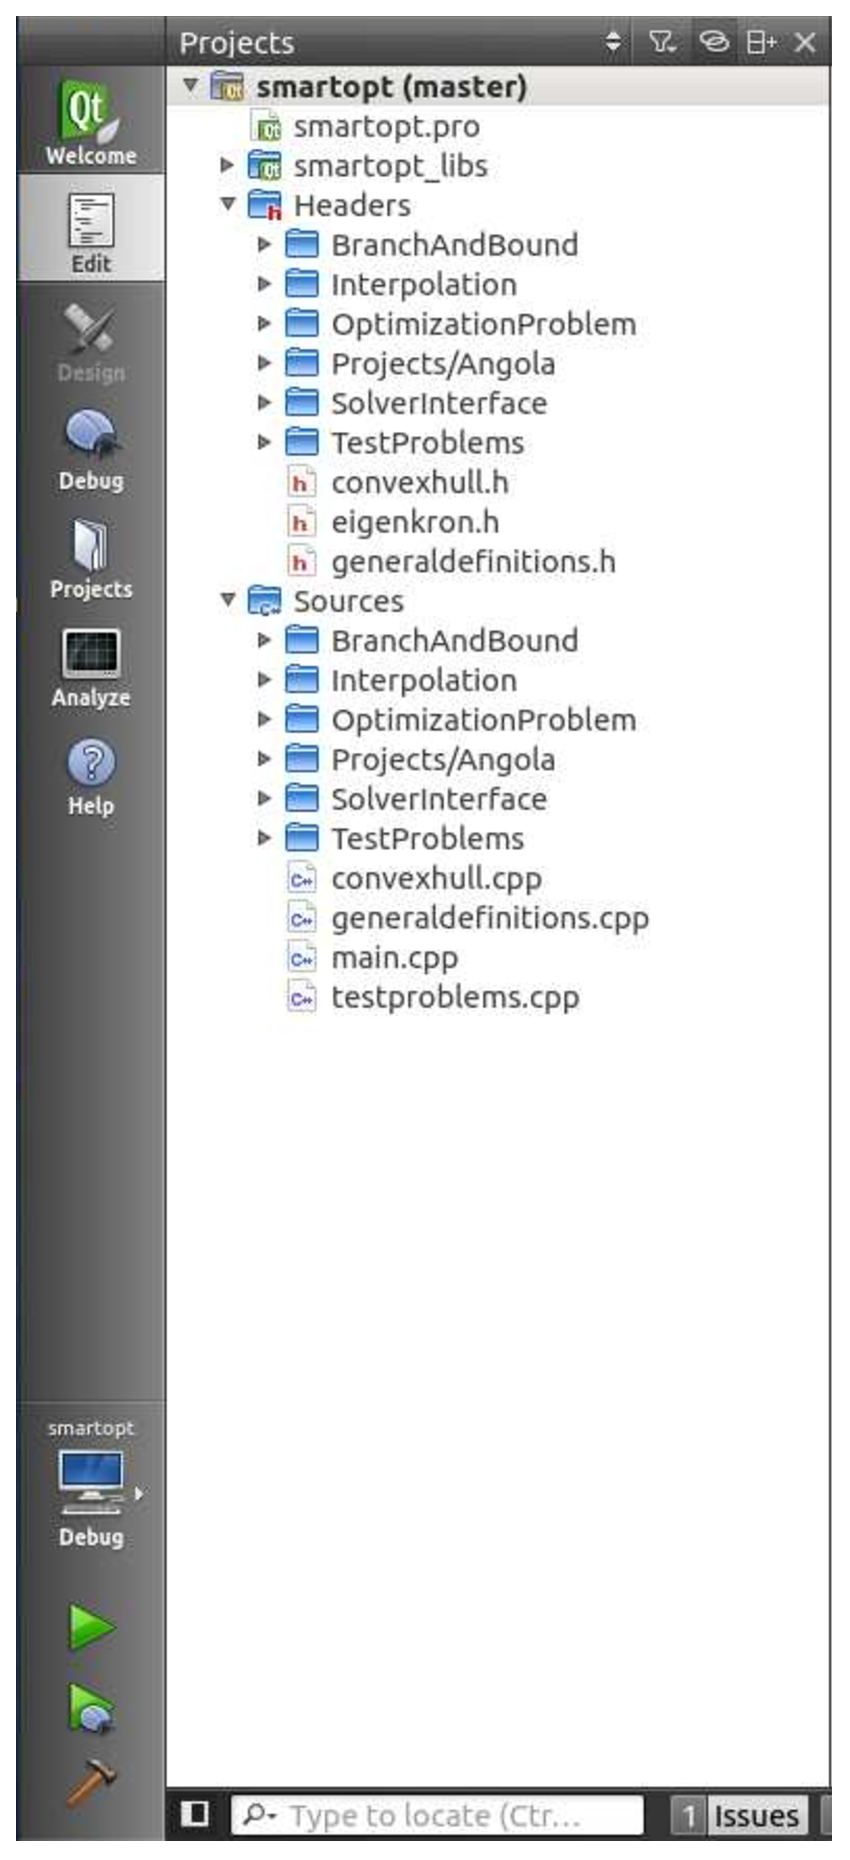
\includegraphics[scale=0.4] {figures/QtCreator.eps}
  \caption{Folder structure in the \solvername\ code, as shown in Qt Creator:
  
  	\textbf{BranchAndBound:} Contains the code and classes required for the Branch-and-Bound algorithm.
  
  	\textbf{Interpolation:} Contains interpolation functionality. This includes the \class{InterpolationTable} class, the B-spline functionality, and linear interpolation functionality.

	\textbf{OptimizationProblem:} Contains the classes required to formulate the optimization problem, that is, the classes which describe constraints and objective functions.

	\textbf{SolverInterface:} Contains the code which translates the optimization problem desribed by the constraint and objective function classes into the format required by the different solvers used (Ipopt, Bonmin, Nomad).

	\textbf{TestProblems:} Contains a framework for testing and some testing problems (including the examples in chapter \ref{sec:examples}).
}
\end{SCfigure}
In Qt Creator, the .cpp and header files are automatically placed in separate folders project tree view, even though they are stored in the same actual folder. When working on a file in the editor, pressing the F4 key conveniently switches between the .cpp and header file.

In addition to the folders described above, some additional files deserve some explanation:
\begin{itemize}
\item
\texttt{smartopt.pro} is the \solvername\ project file, and the project is opened in Qt Creator by opening this file. What it actually contains is the information required by qmake to build the application.
\item
The folder \texttt{smartopt\_libs} contains the \texttt{smartopt\_libs.pri} file which contains library include paths to the various libraries used by \solvername. It also specifies some qmake configuration and compile flags.
\item
\texttt{generaldefinitions.h} and \texttt{generaldefinitions.cpp} contain some general functionality like typedefs, enums, printing functions and transformations, which is reused throughout the code. 
\item
The \texttt{main.cpp} file contains the \texttt{main()} function.
\end{itemize}